\chapter{Figures}

\vspace{4in}
\;

\begin{figure}[H]
  \begin{center}
    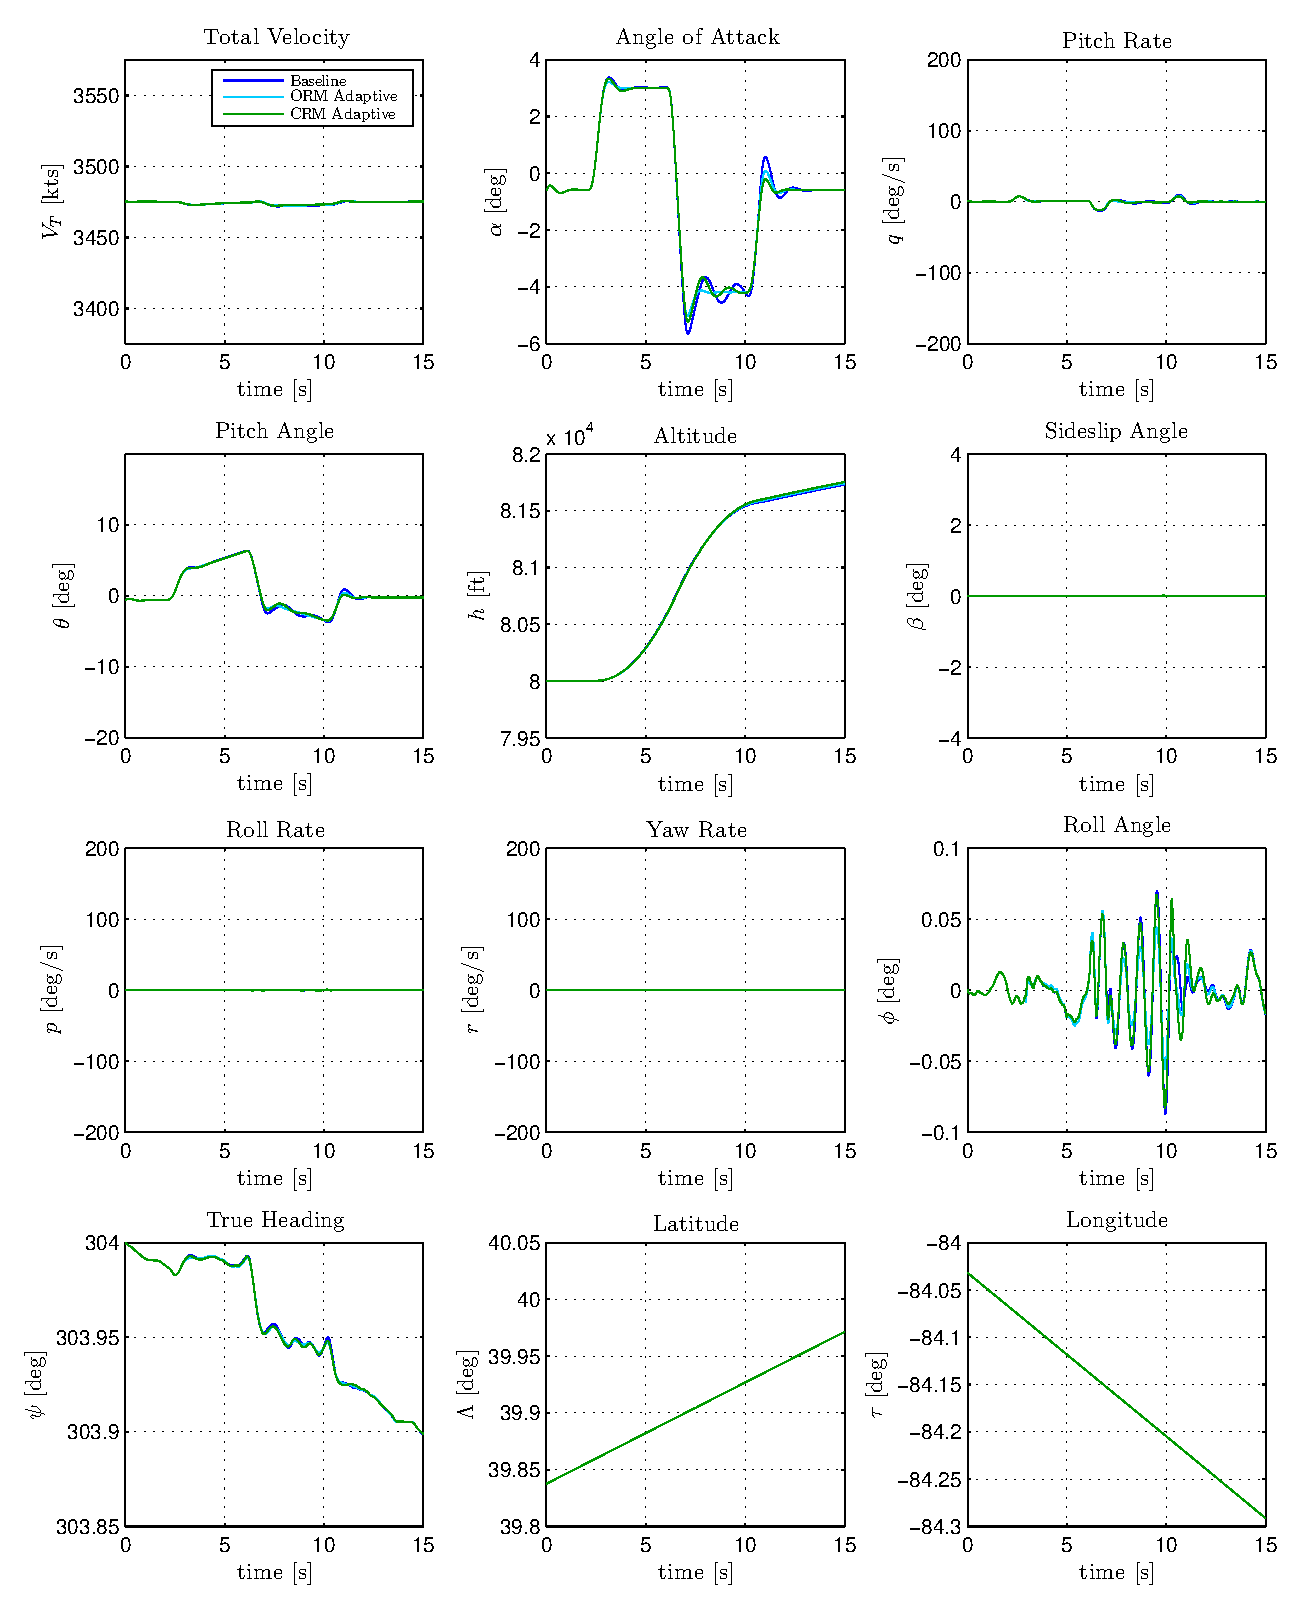
\includegraphics[width=6.5in]{\figurepath/state_longres_cef050b.eps}
    \caption{1A:\ State response for reduced control surface effectiveness: 50\% on all surfaces}
  \end{center}
\end{figure}

\begin{figure}[H]
  \begin{center}
    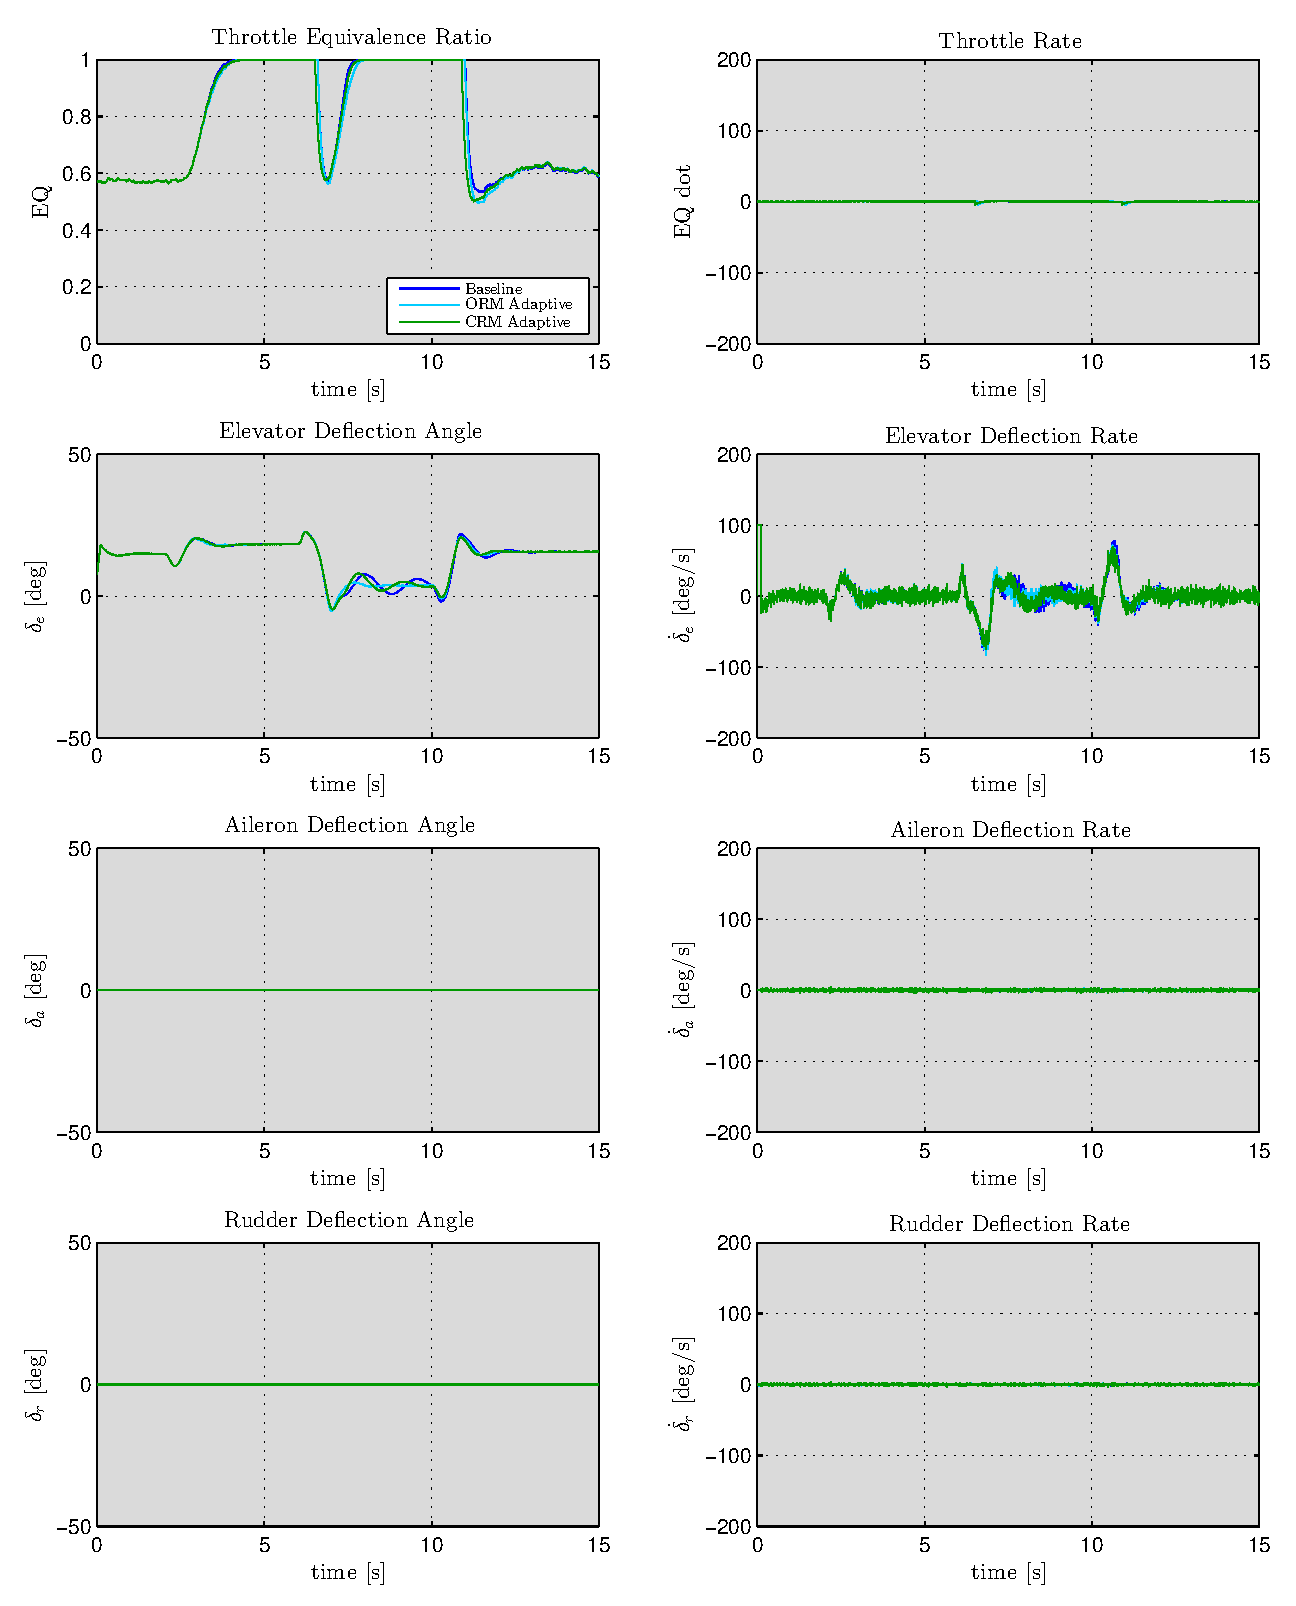
\includegraphics[width=6.5in]{\figurepath/input_longres_cef050b.eps}
    \caption{1A:\ Input response for reduced control surface effectiveness: 50\% on all surfaces}
  \end{center}
\end{figure}

\begin{figure}[H]
  \begin{center}
    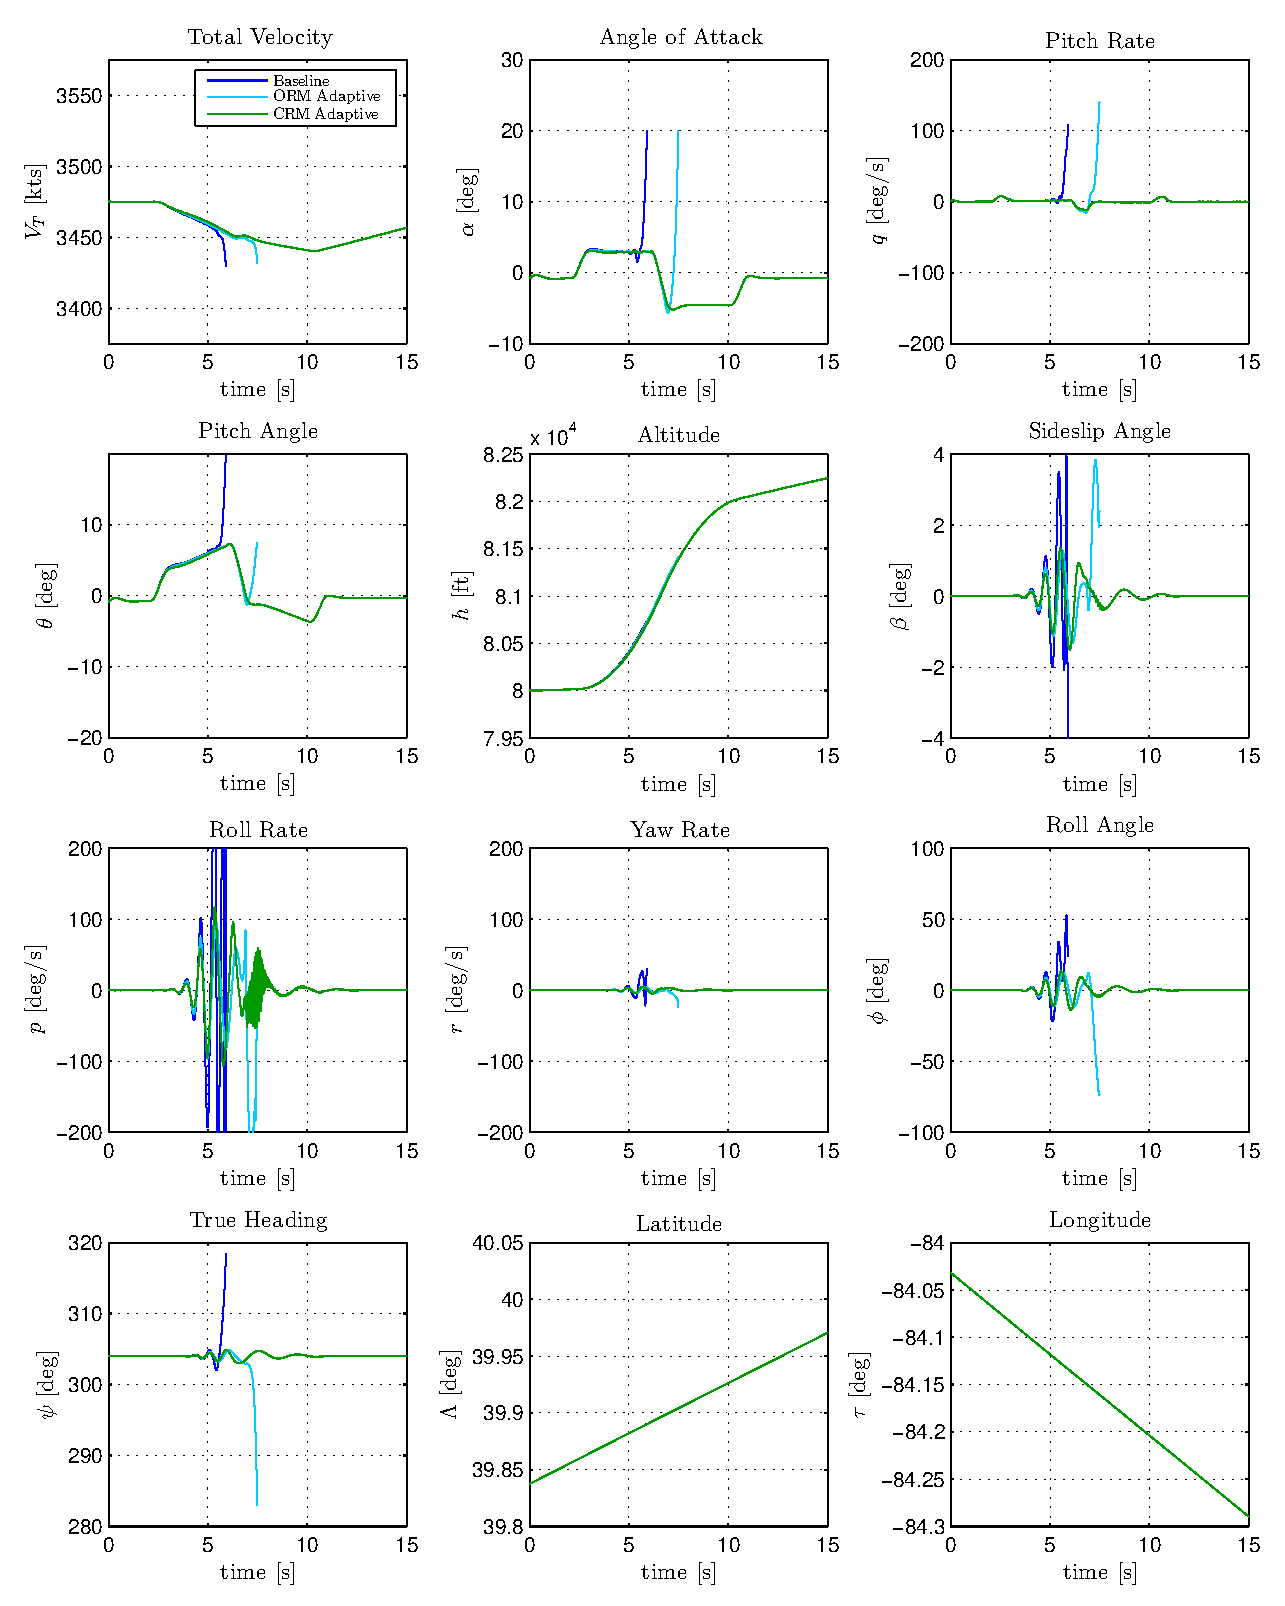
\includegraphics[width=6.5in]{\figurepath/state_longres_cgx090b.eps}
    \caption{1B:\ State response for longitudinal CG shift: -0.9 ft rearward}
  \end{center}
\end{figure}

\begin{figure}[H]
  \begin{center}
    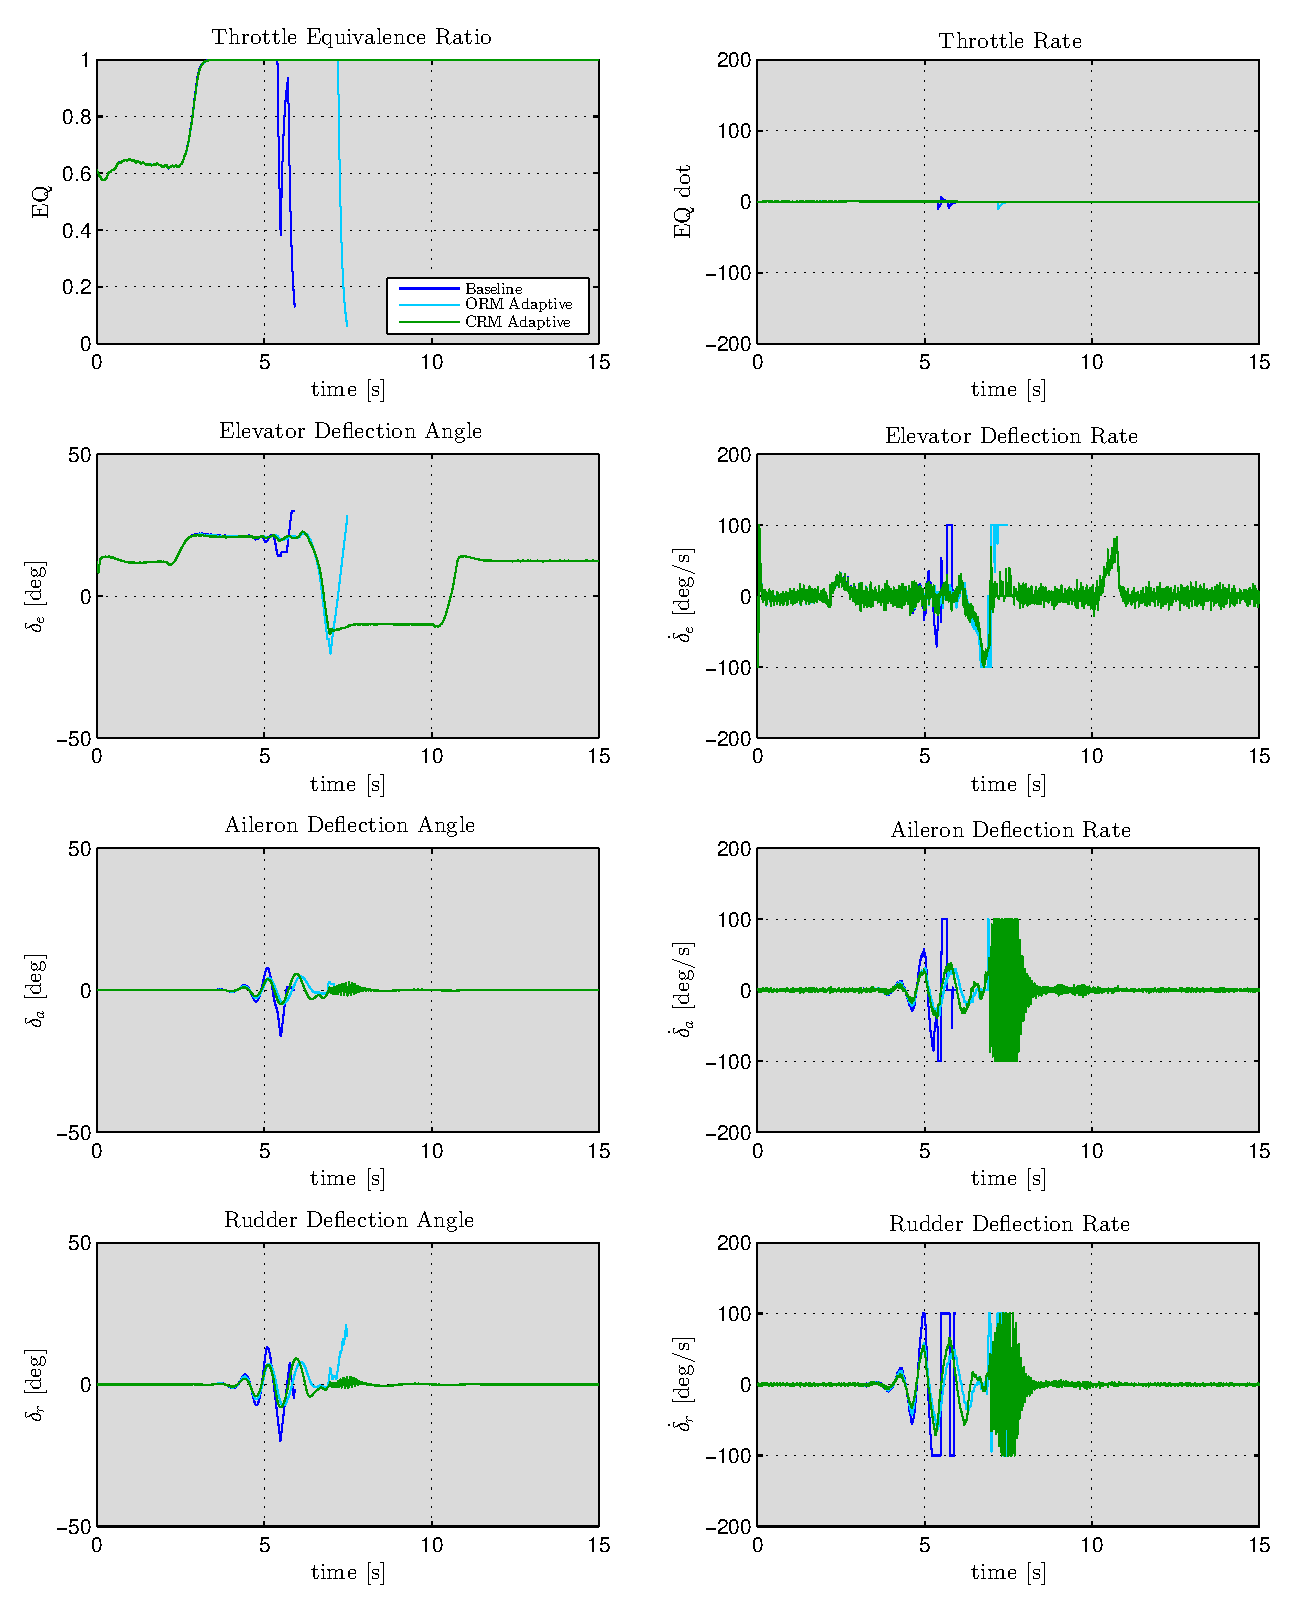
\includegraphics[width=6.5in]{\figurepath/input_longres_cgx090b.eps}
    \caption{1B:\ Input response for longitudinal CG shift: -0.9 ft rearward}
  \end{center}
\end{figure}

\begin{figure}[H]
  \begin{center}
    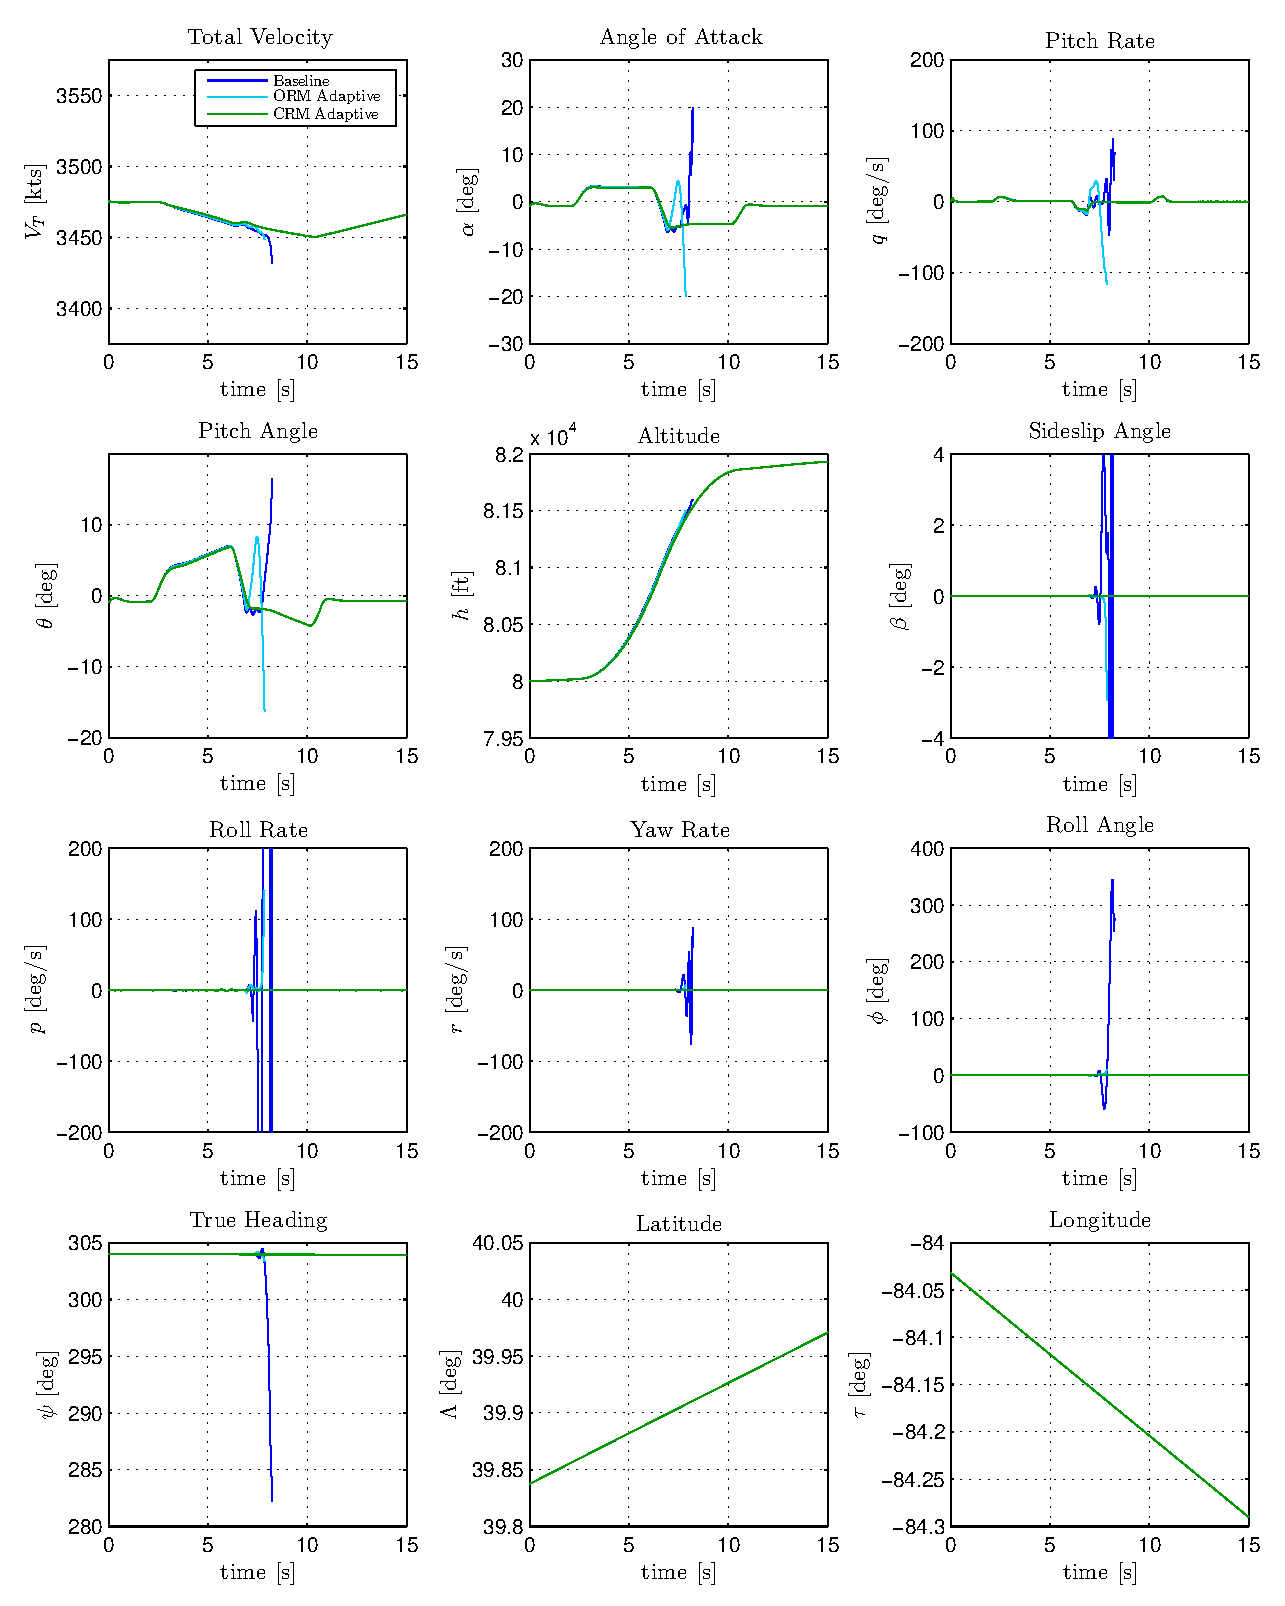
\includegraphics[width=6.5in]{\figurepath/state_longres_cma400b.eps}
    \caption{1C:\ State response for pitching moment coefficient scaled $4\times$}
  \end{center}
\end{figure}

\begin{figure}[H]
  \begin{center}
    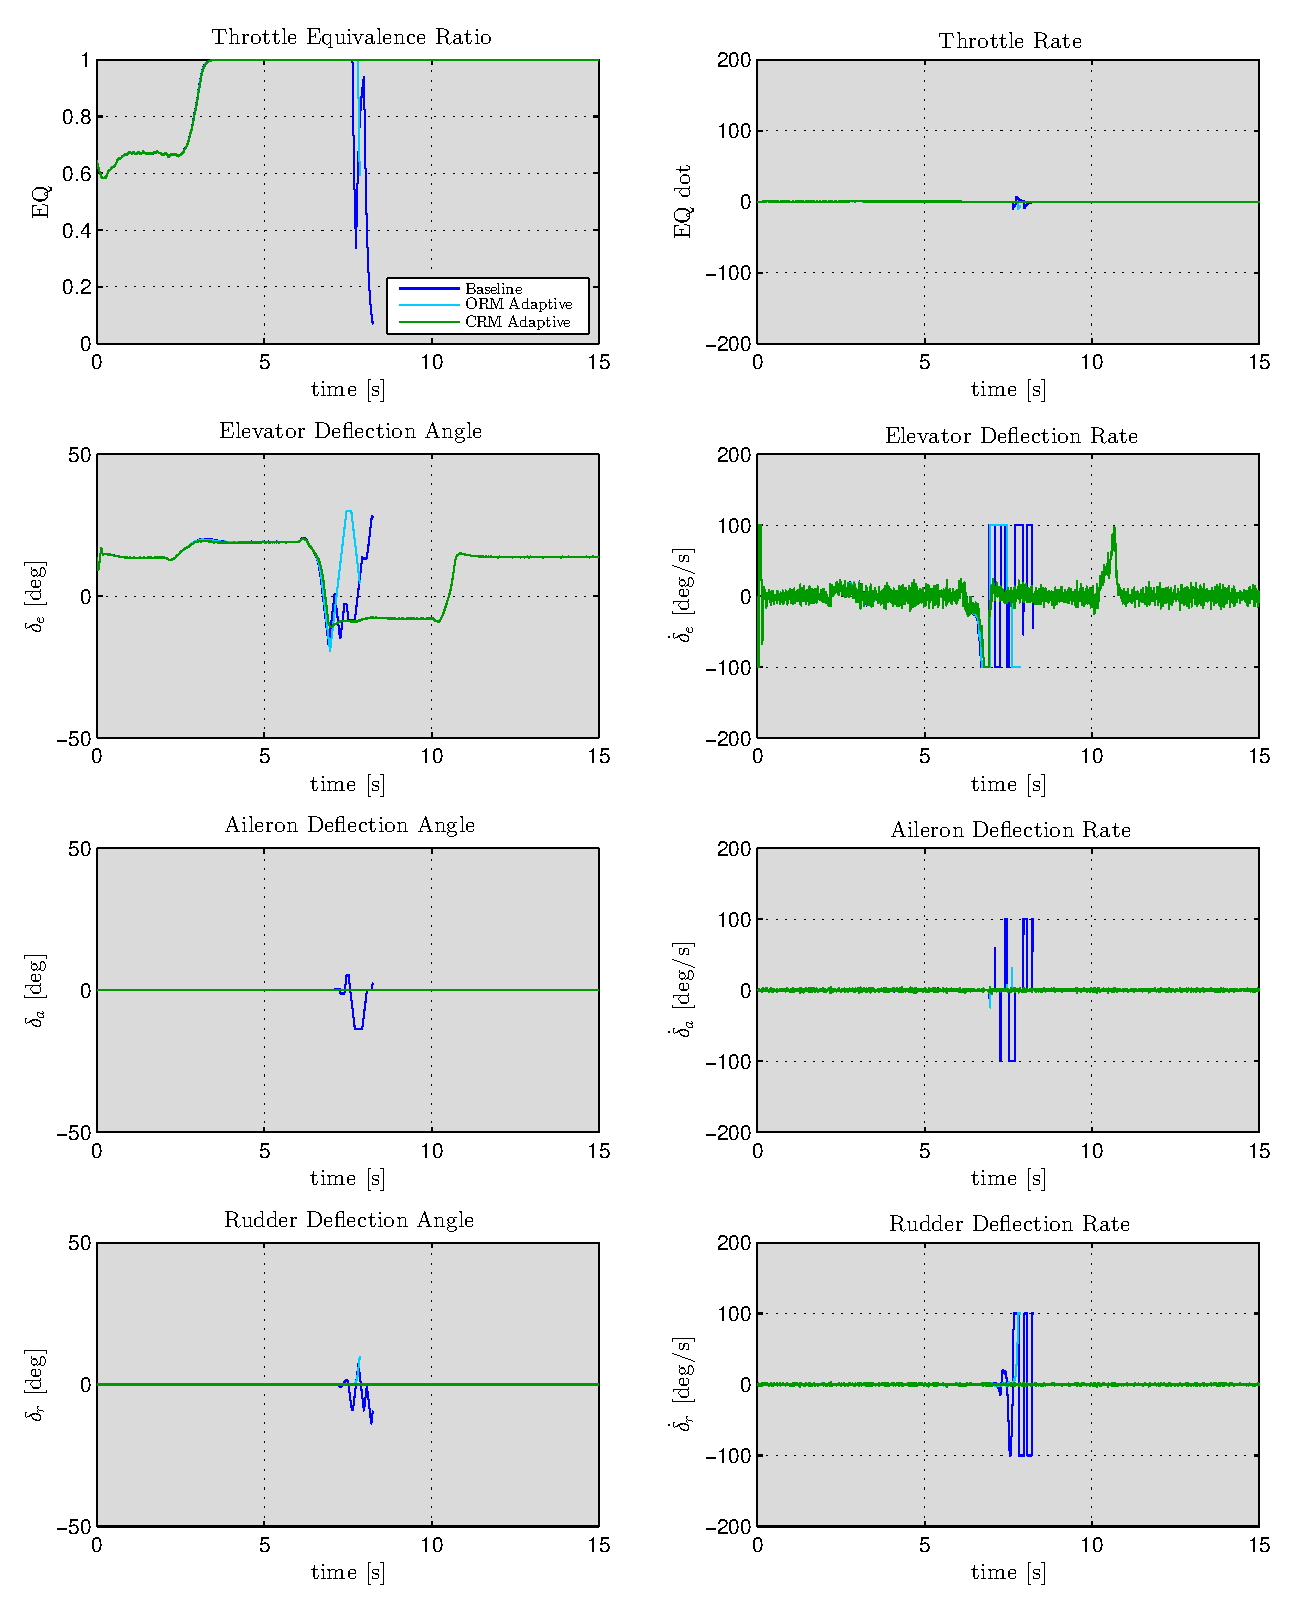
\includegraphics[width=6.5in]{\figurepath/input_longres_cma400b.eps}
    \caption{1C:\ Input response for pitching moment coefficient scaled $4\times$}
  \end{center}
\end{figure}

\begin{figure}[H]
  \begin{center}
    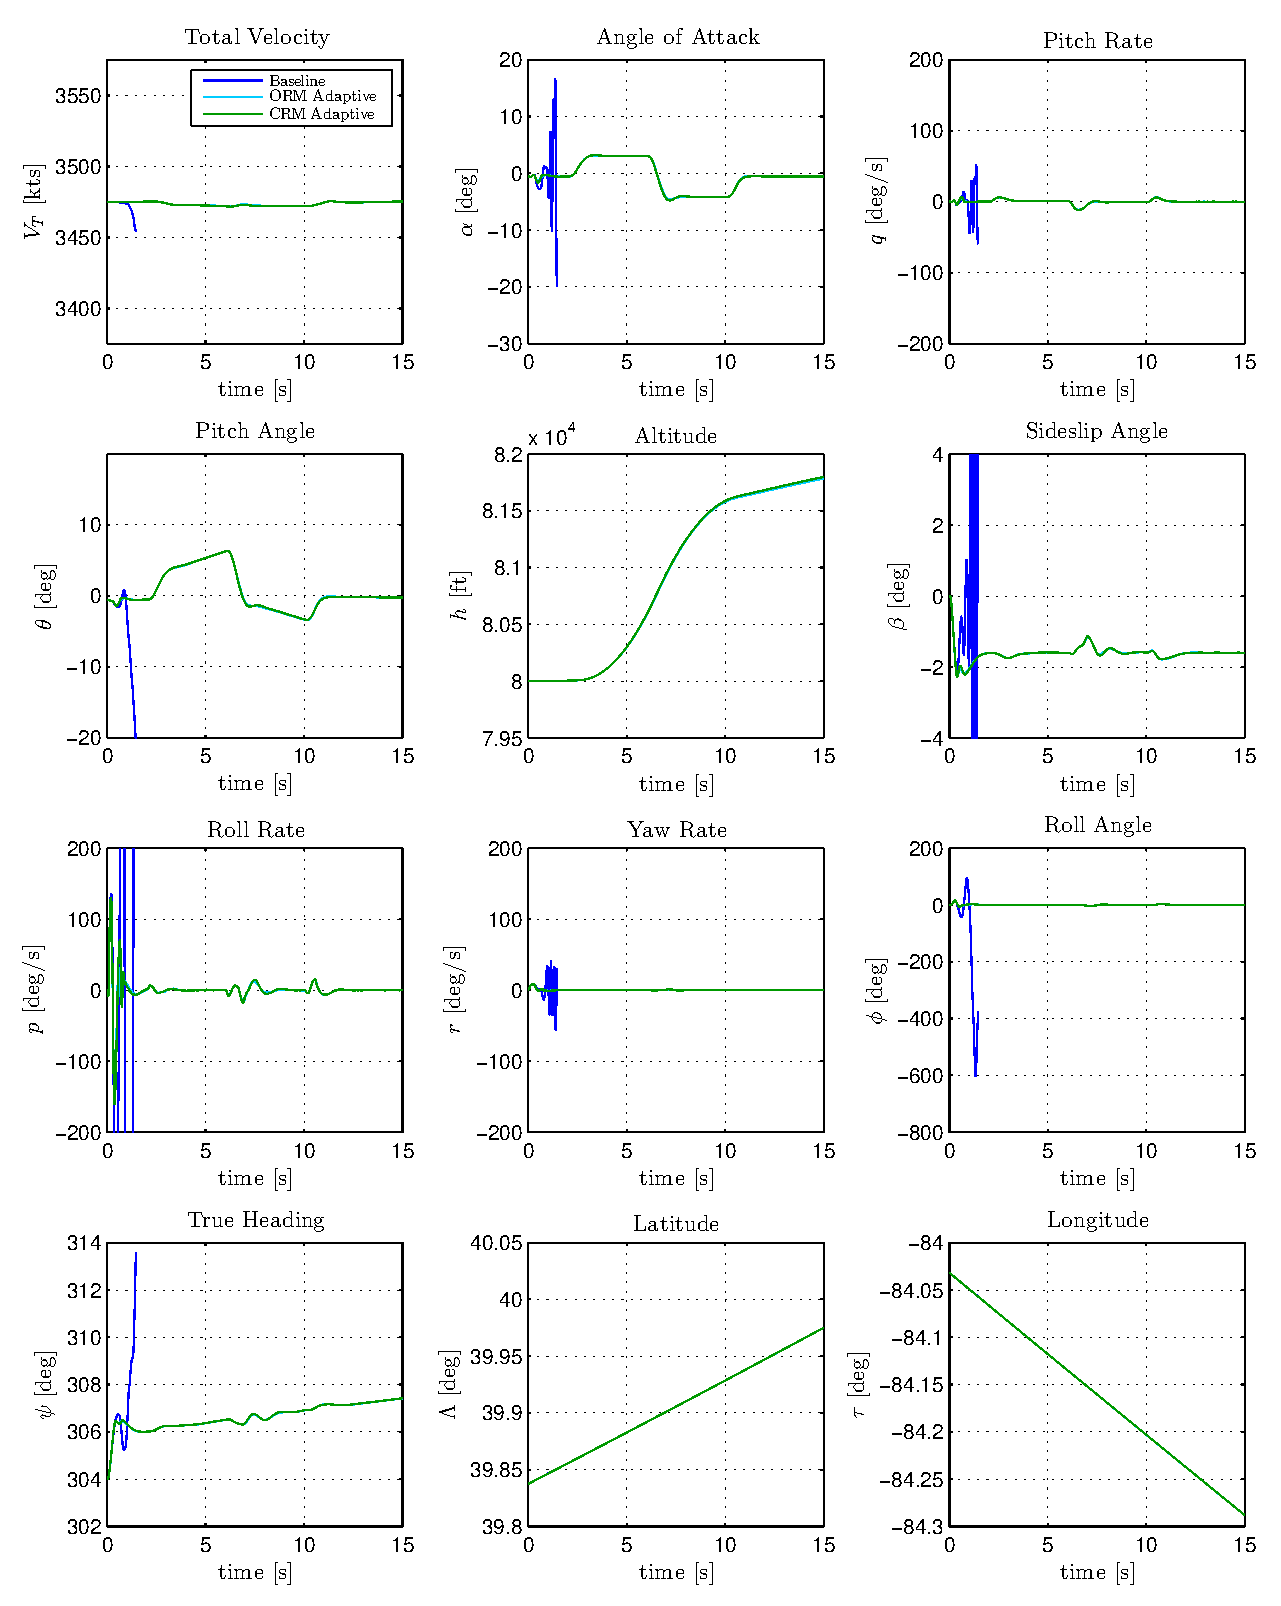
\includegraphics[width=6.5in]{\figurepath/state_longres_bia016b.eps}
    \caption{1D:\ State response for sensor bias of $+1.6$ degrees on sideslip measurement}
  \end{center}
\end{figure}

\begin{figure}[H]
  \begin{center}
    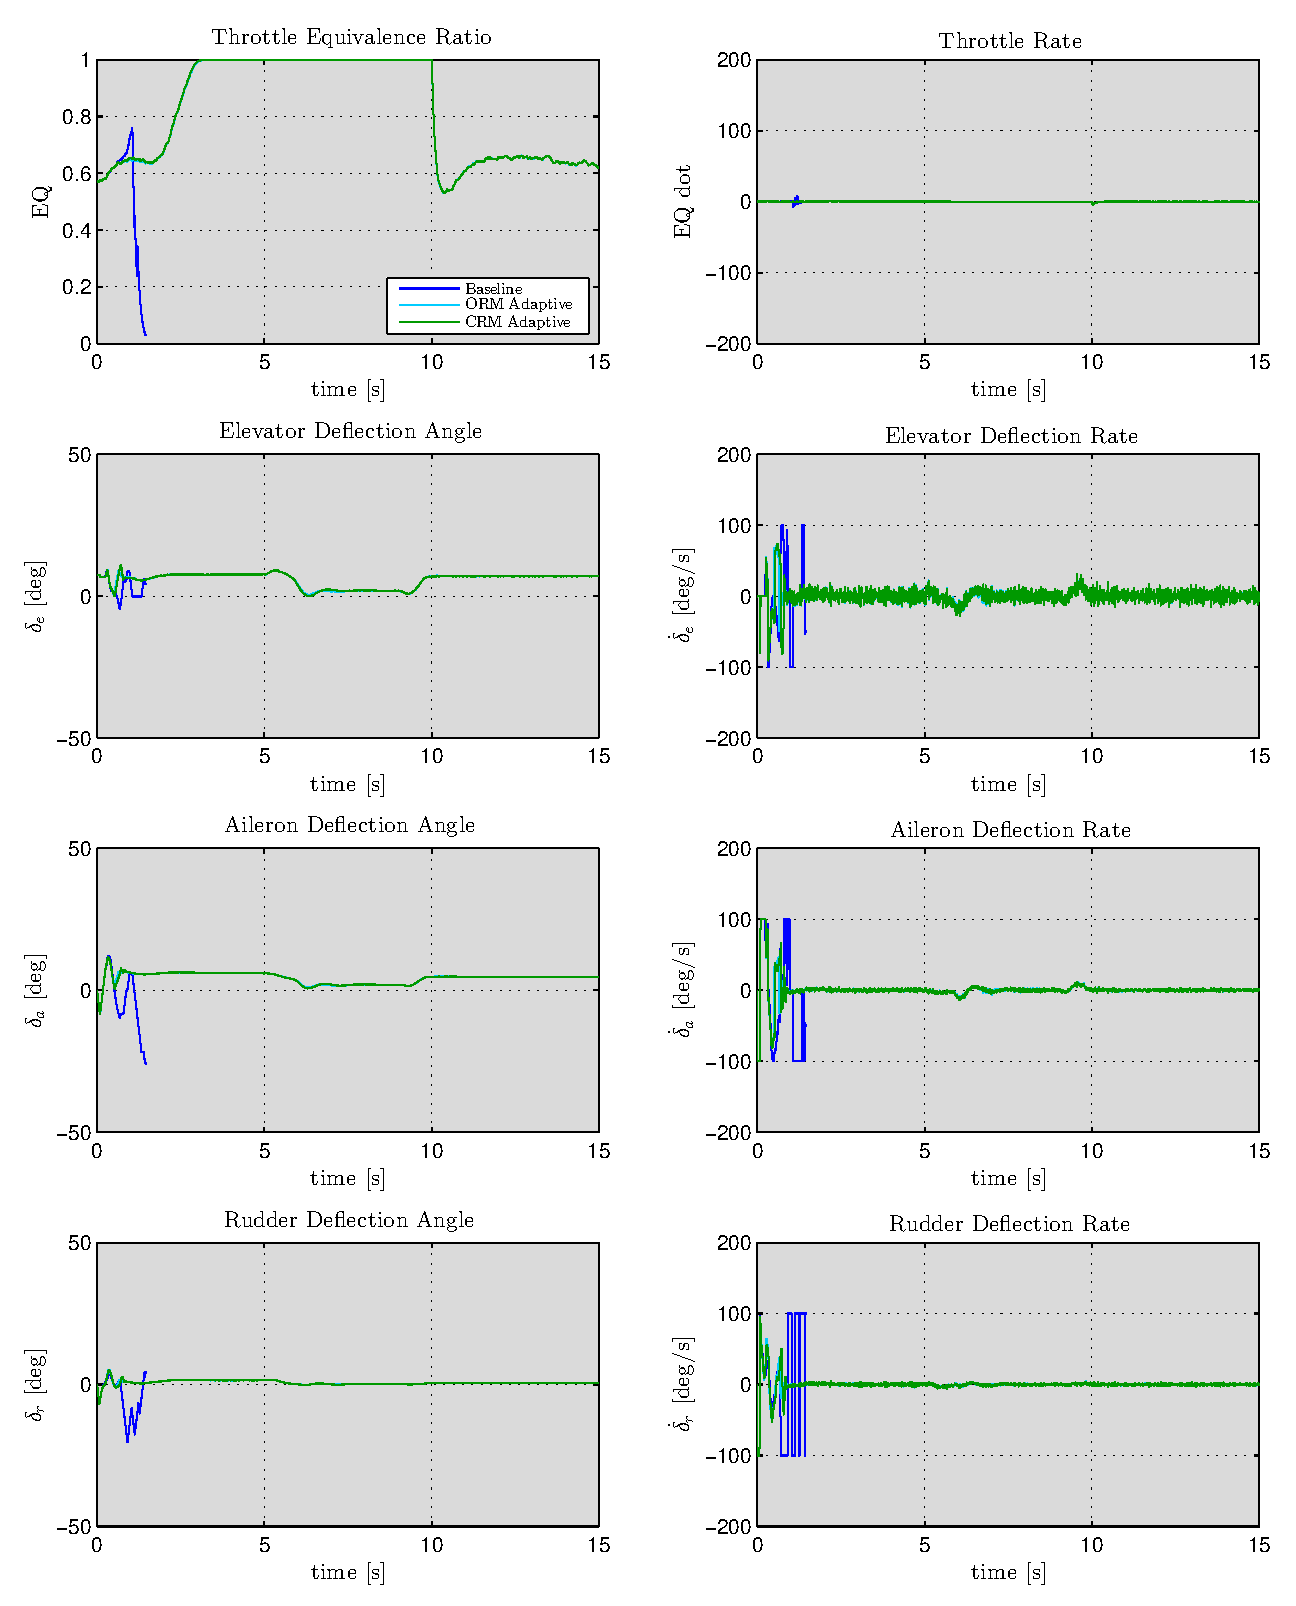
\includegraphics[width=6.5in]{\figurepath/input_longres_bia016.eps}
    \caption{1D:\ State response for sensor bias of $+1.6$ degrees on sideslip measurement}
  \end{center}
\end{figure}

\begin{figure}[H]
  \begin{center}
    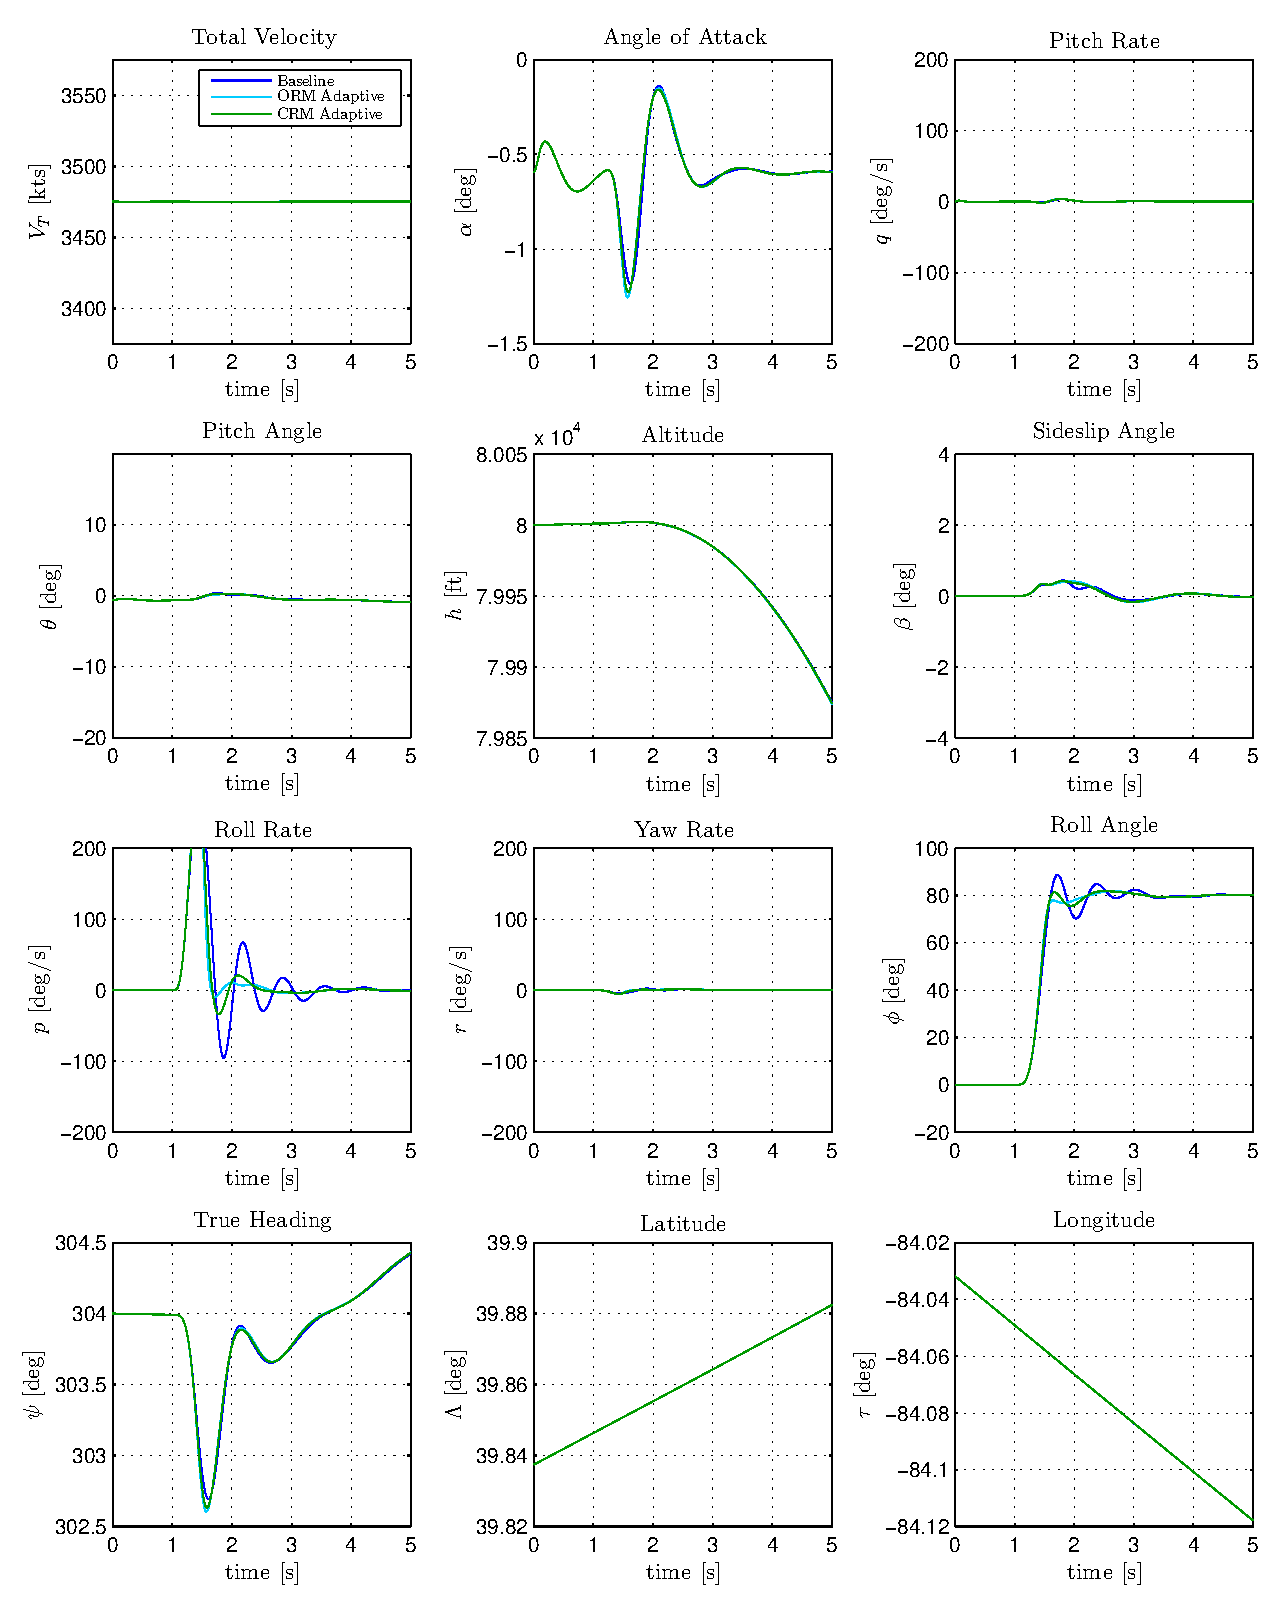
\includegraphics[width=6.5in]{\figurepath/state_latrres_cef050b.eps}
    \caption{2A:\ State response with 50\% control surface effectiveness on all surfaces}
  \end{center}
\end{figure}

\begin{figure}[H]
  \begin{center}
    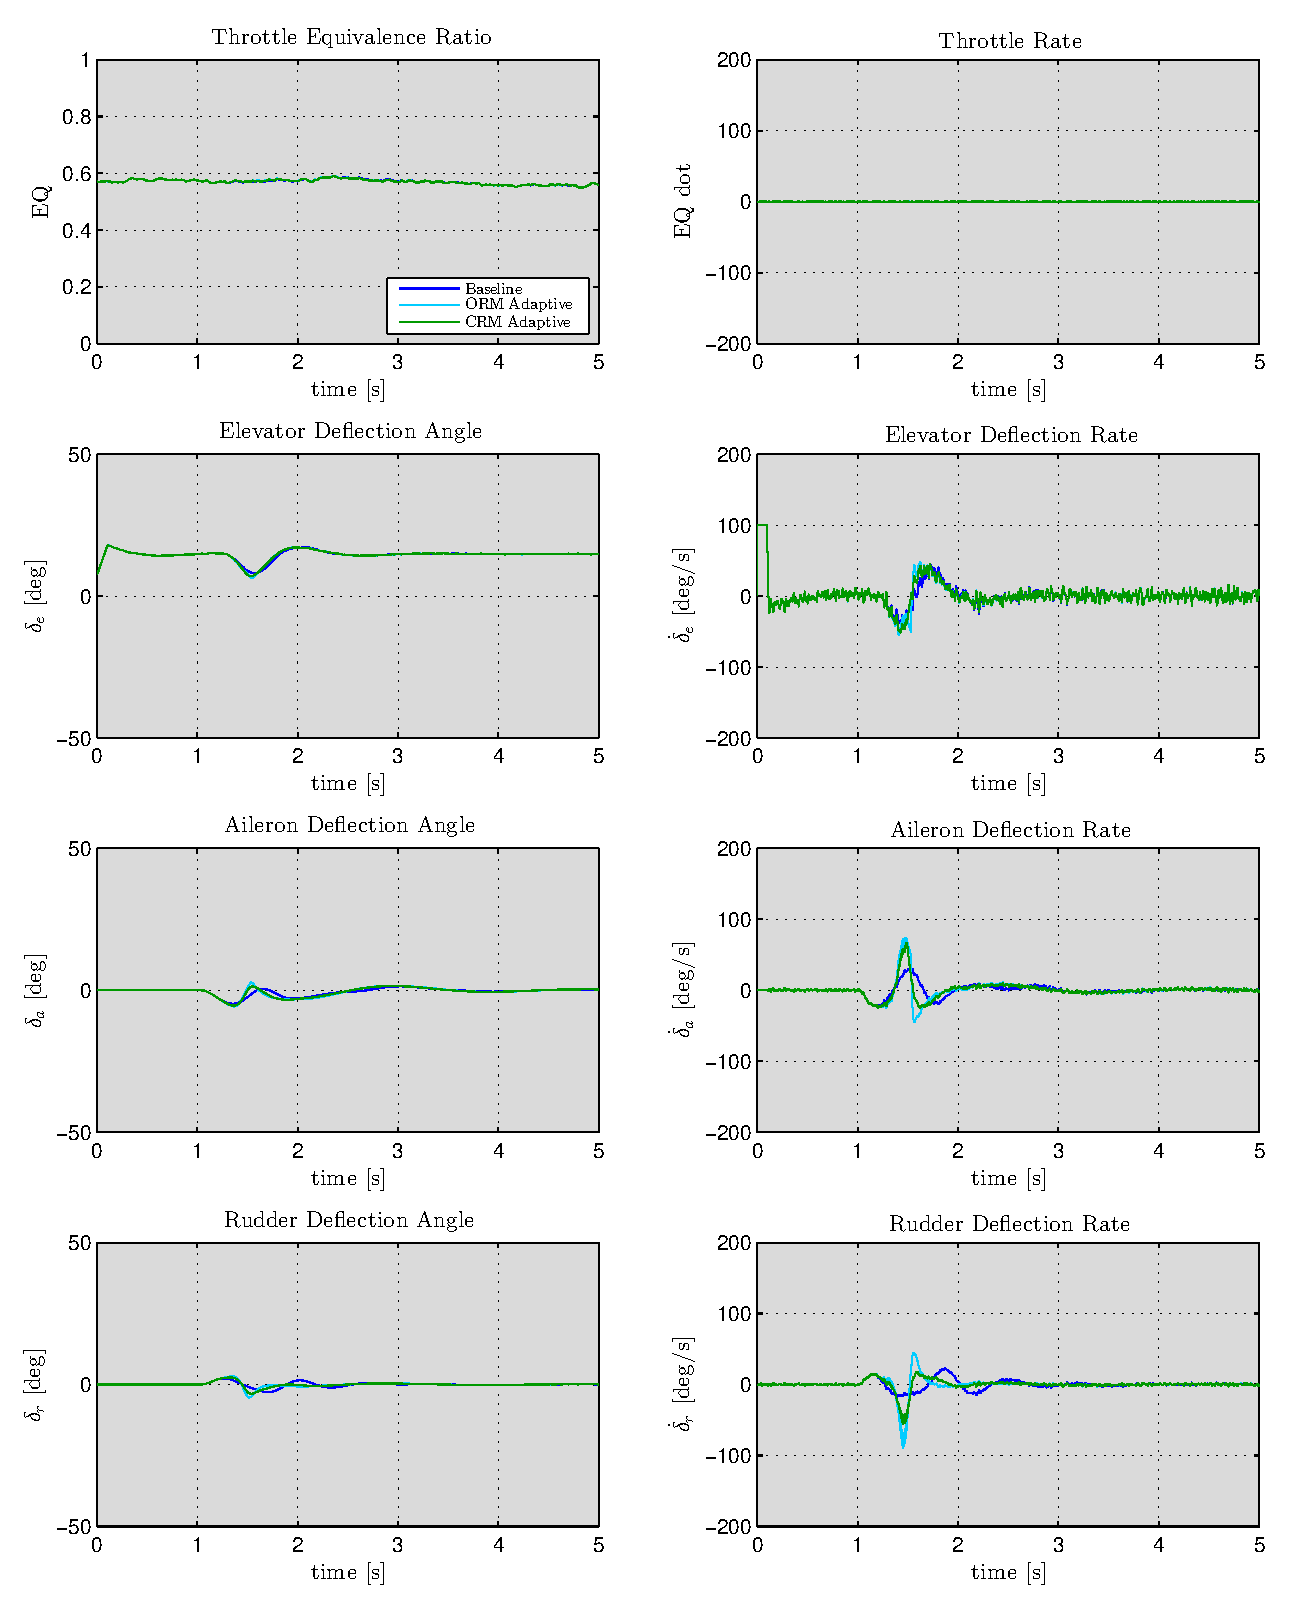
\includegraphics[width=6.5in]{\figurepath/input_latrres_cef050b.eps}
    \caption{2A:\ Input response with 50\% control surface effectiveness on all surfaces}
  \end{center}
\end{figure}

\begin{figure}[H]
  \begin{center}
    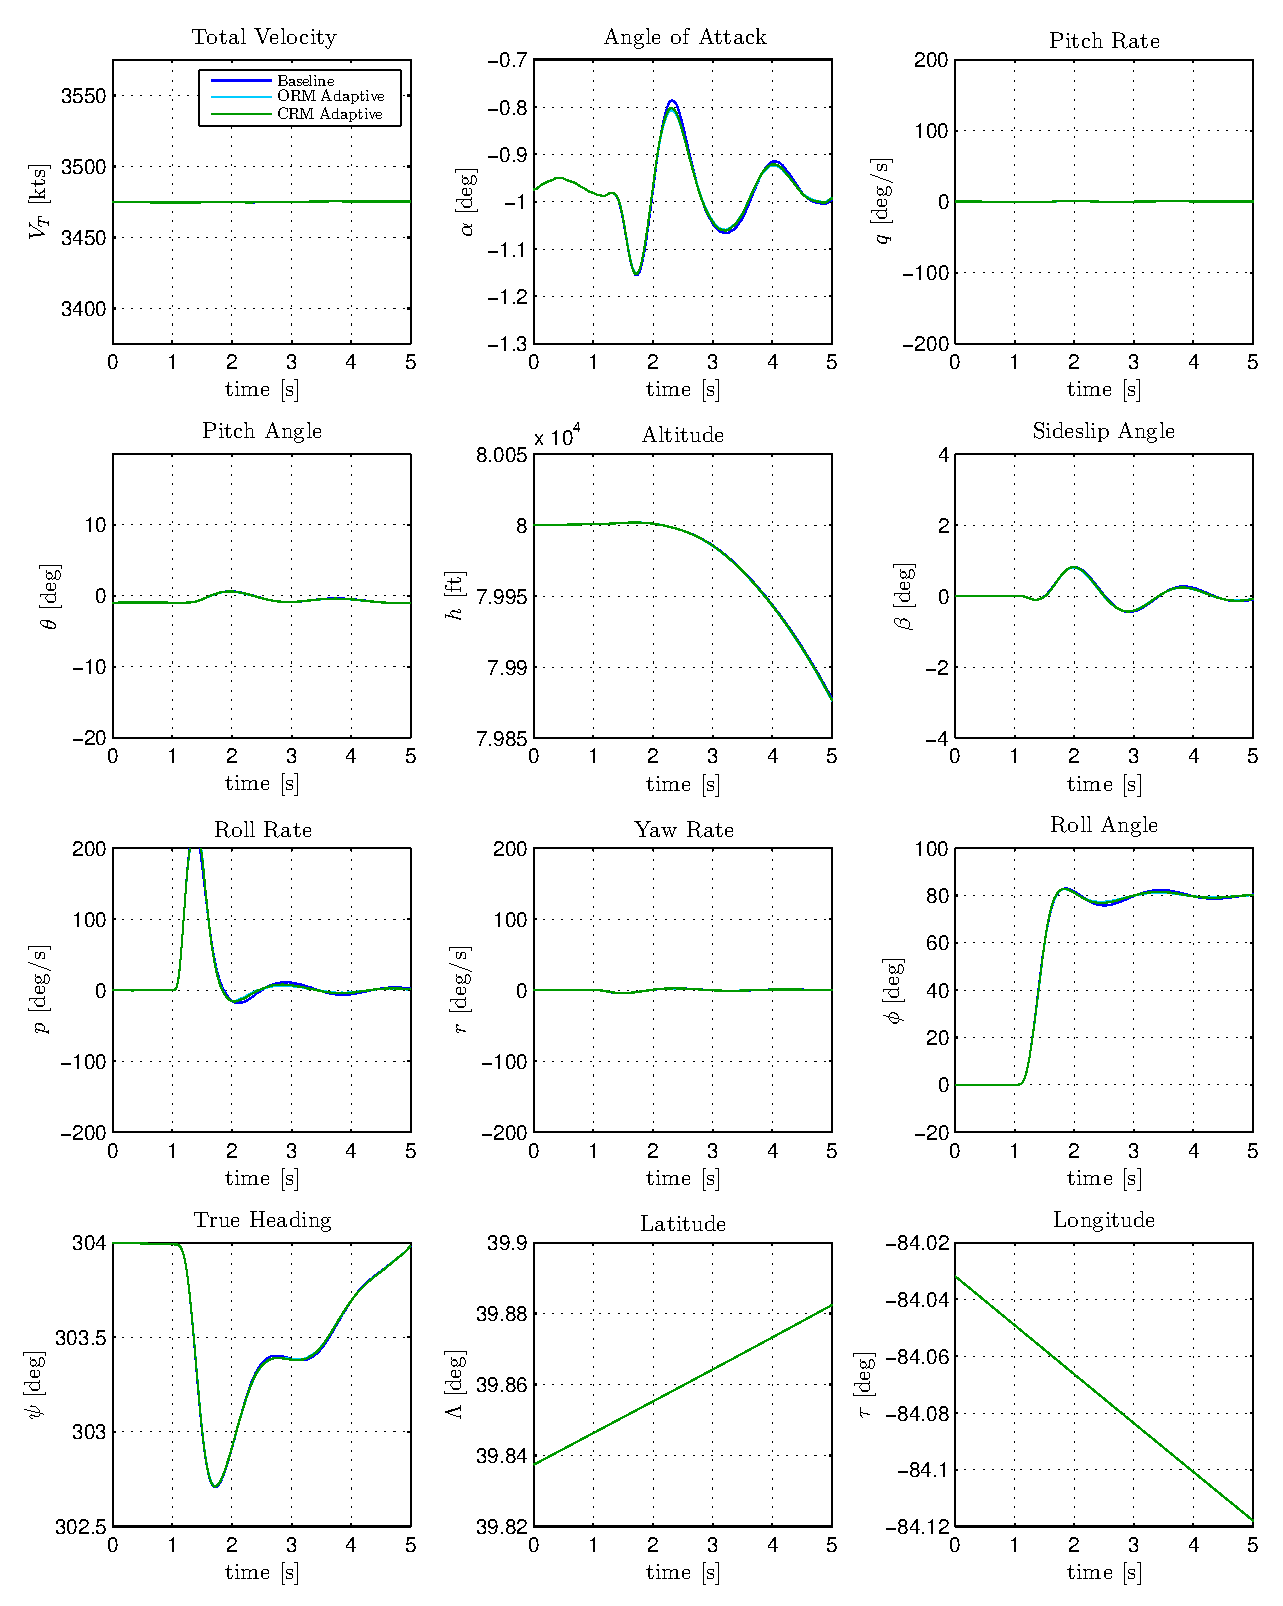
\includegraphics[width=6.5in]{\figurepath/state_latrres_cgx160b.eps}
    \caption{2B:\ State response with longitudinal CG shift: -1.6 ft rearward}
  \end{center}
\end{figure}

\begin{figure}[H]
  \begin{center}
    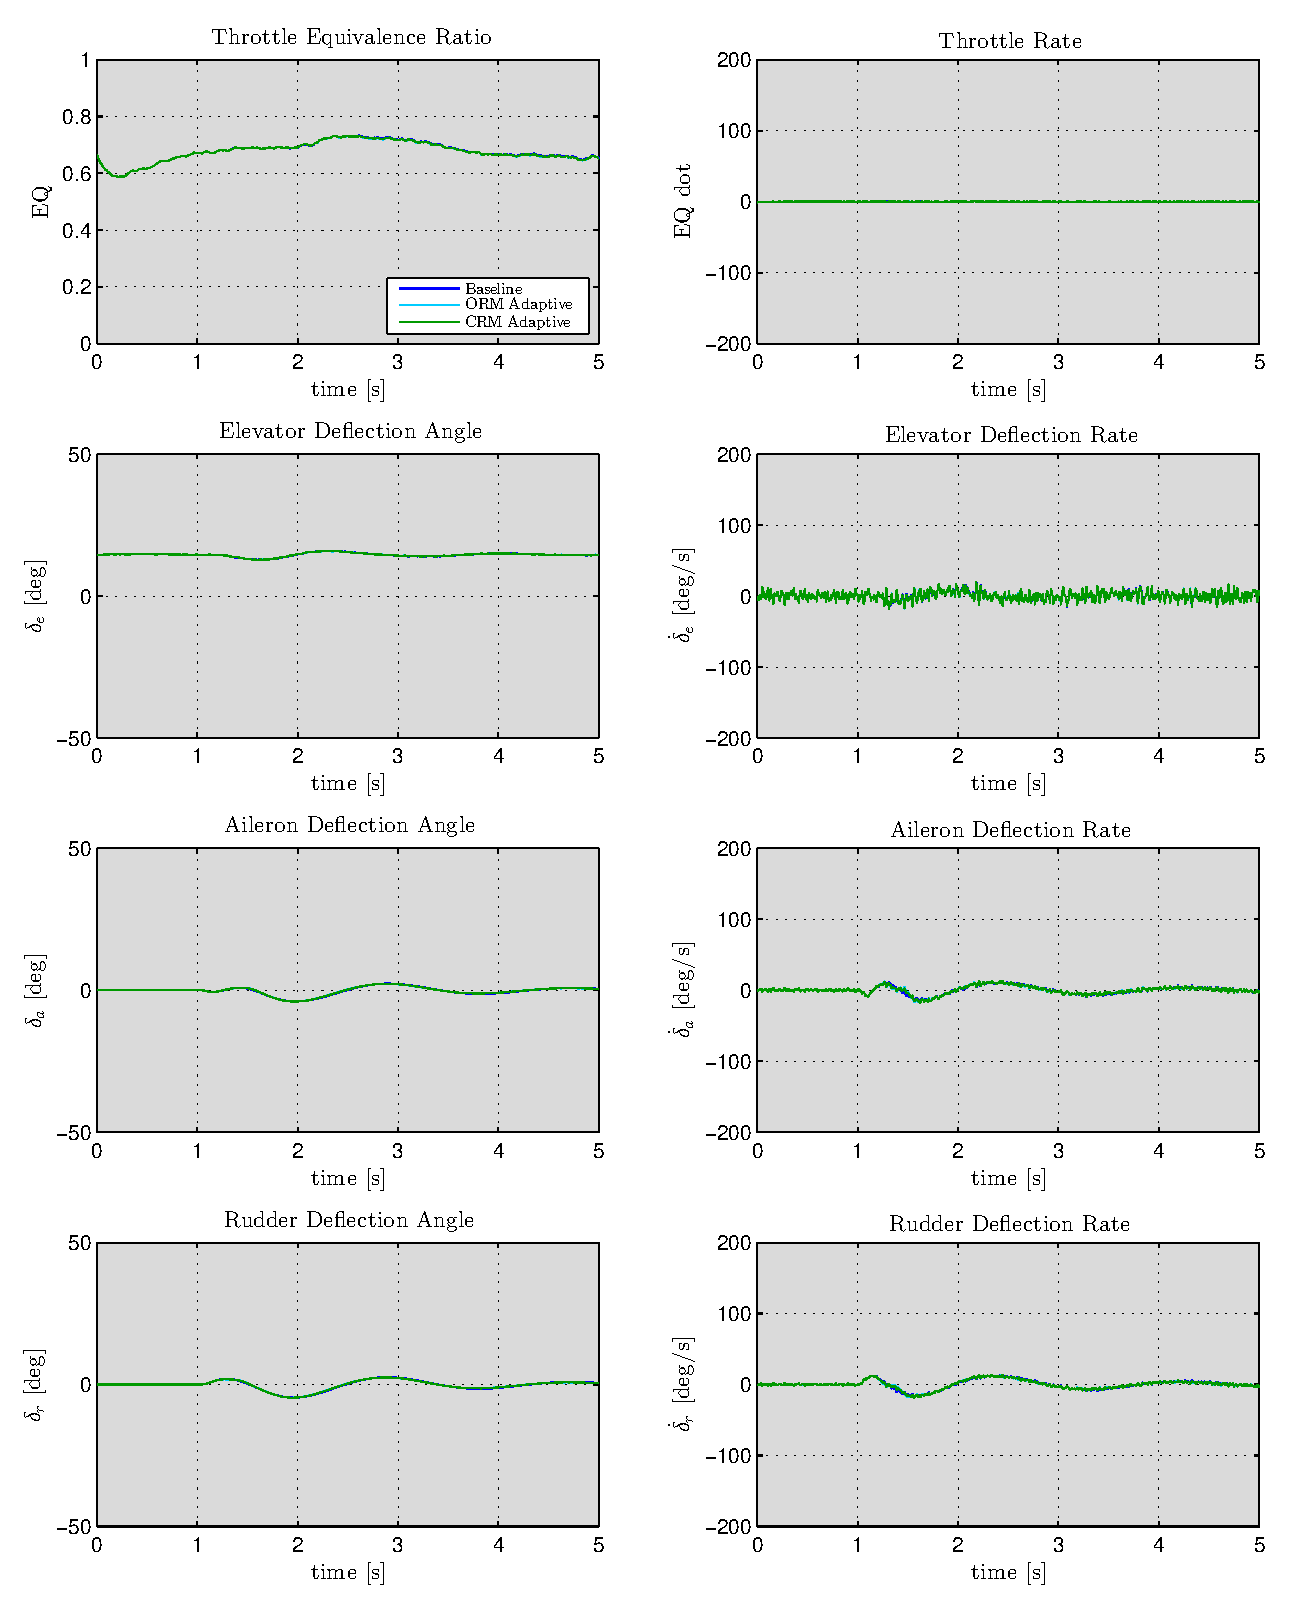
\includegraphics[width=6.5in]{\figurepath/input_latrres_cgx160b.eps}
    \caption{2B:\ State response with longitudinal CG shift: -1.6 ft rearward}
  \end{center}
\end{figure}

\begin{figure}[H]
  \begin{center}
    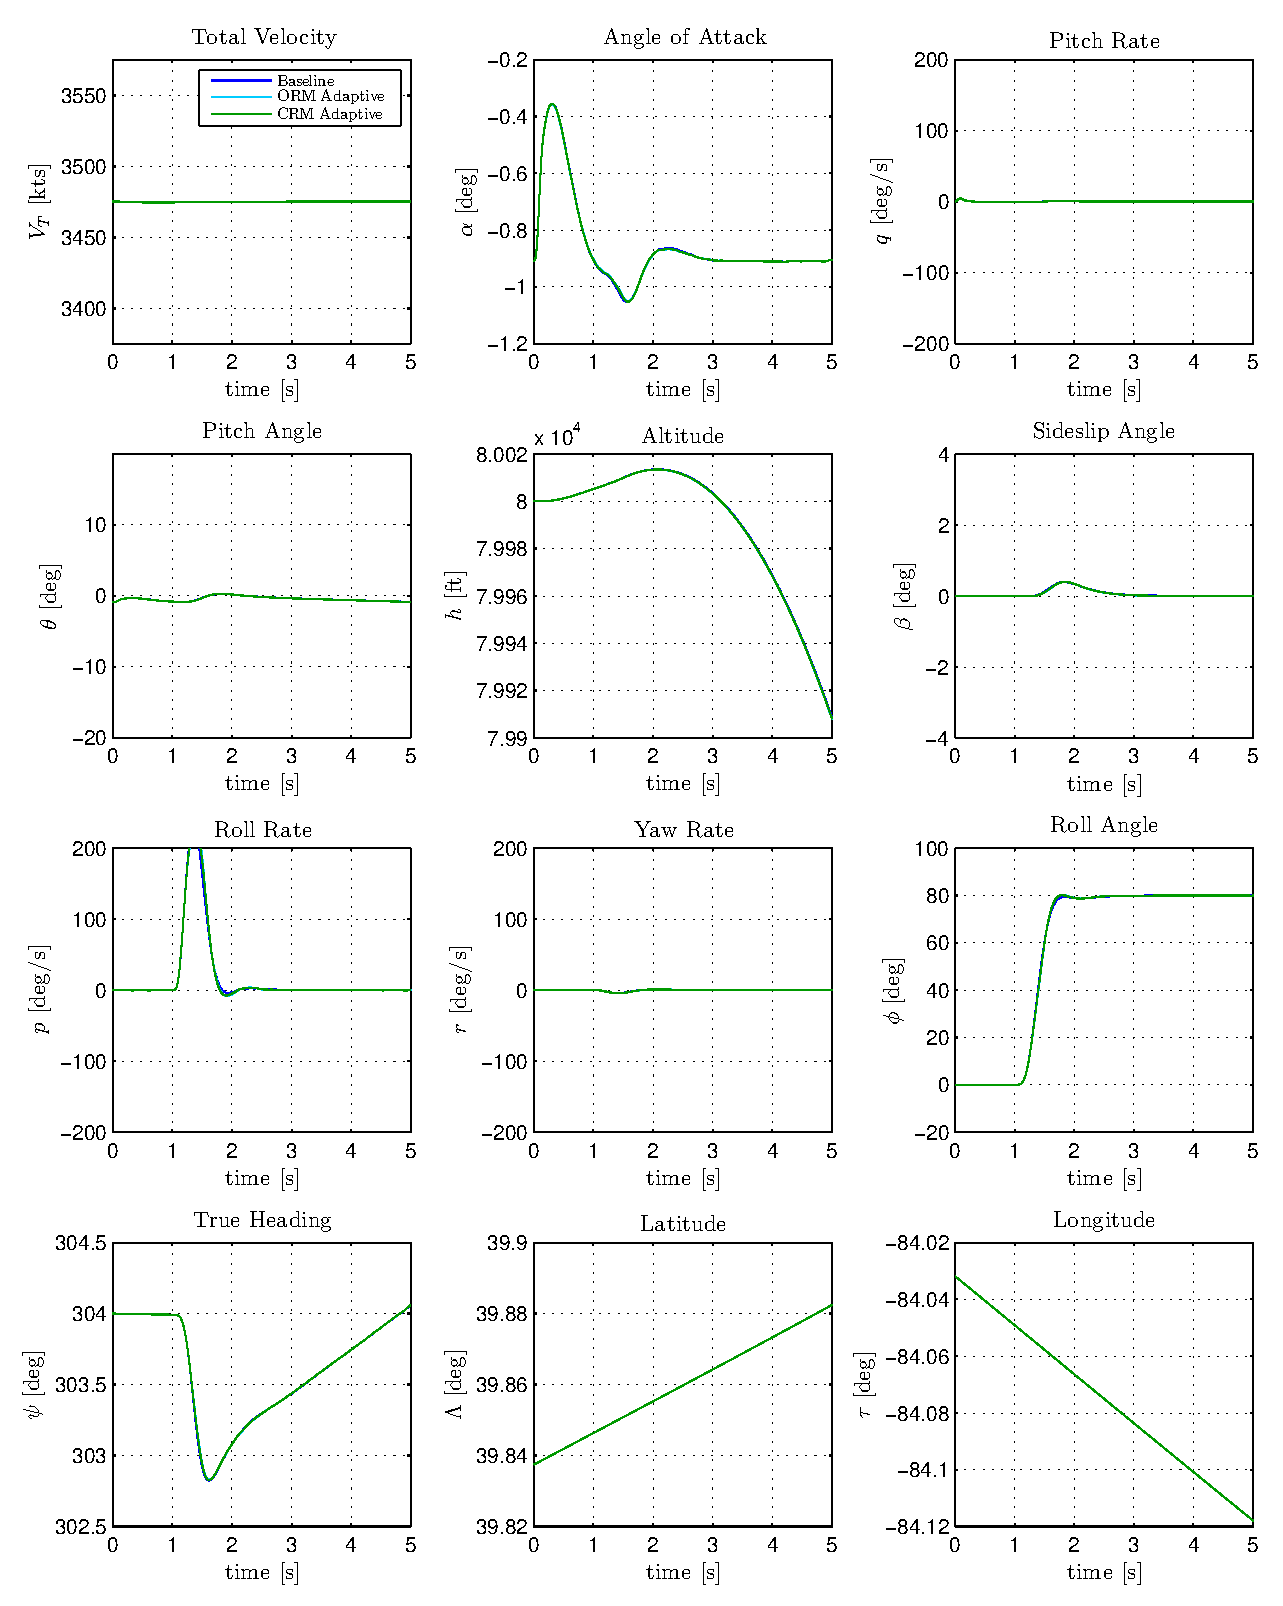
\includegraphics[width=6.5in]{\figurepath/state_latrres_cma400b.eps}
    \caption{2C:\ State response for pitching moment coefficient scaled $4\times$}
  \end{center}
\end{figure}

\begin{figure}[H]
  \begin{center}
    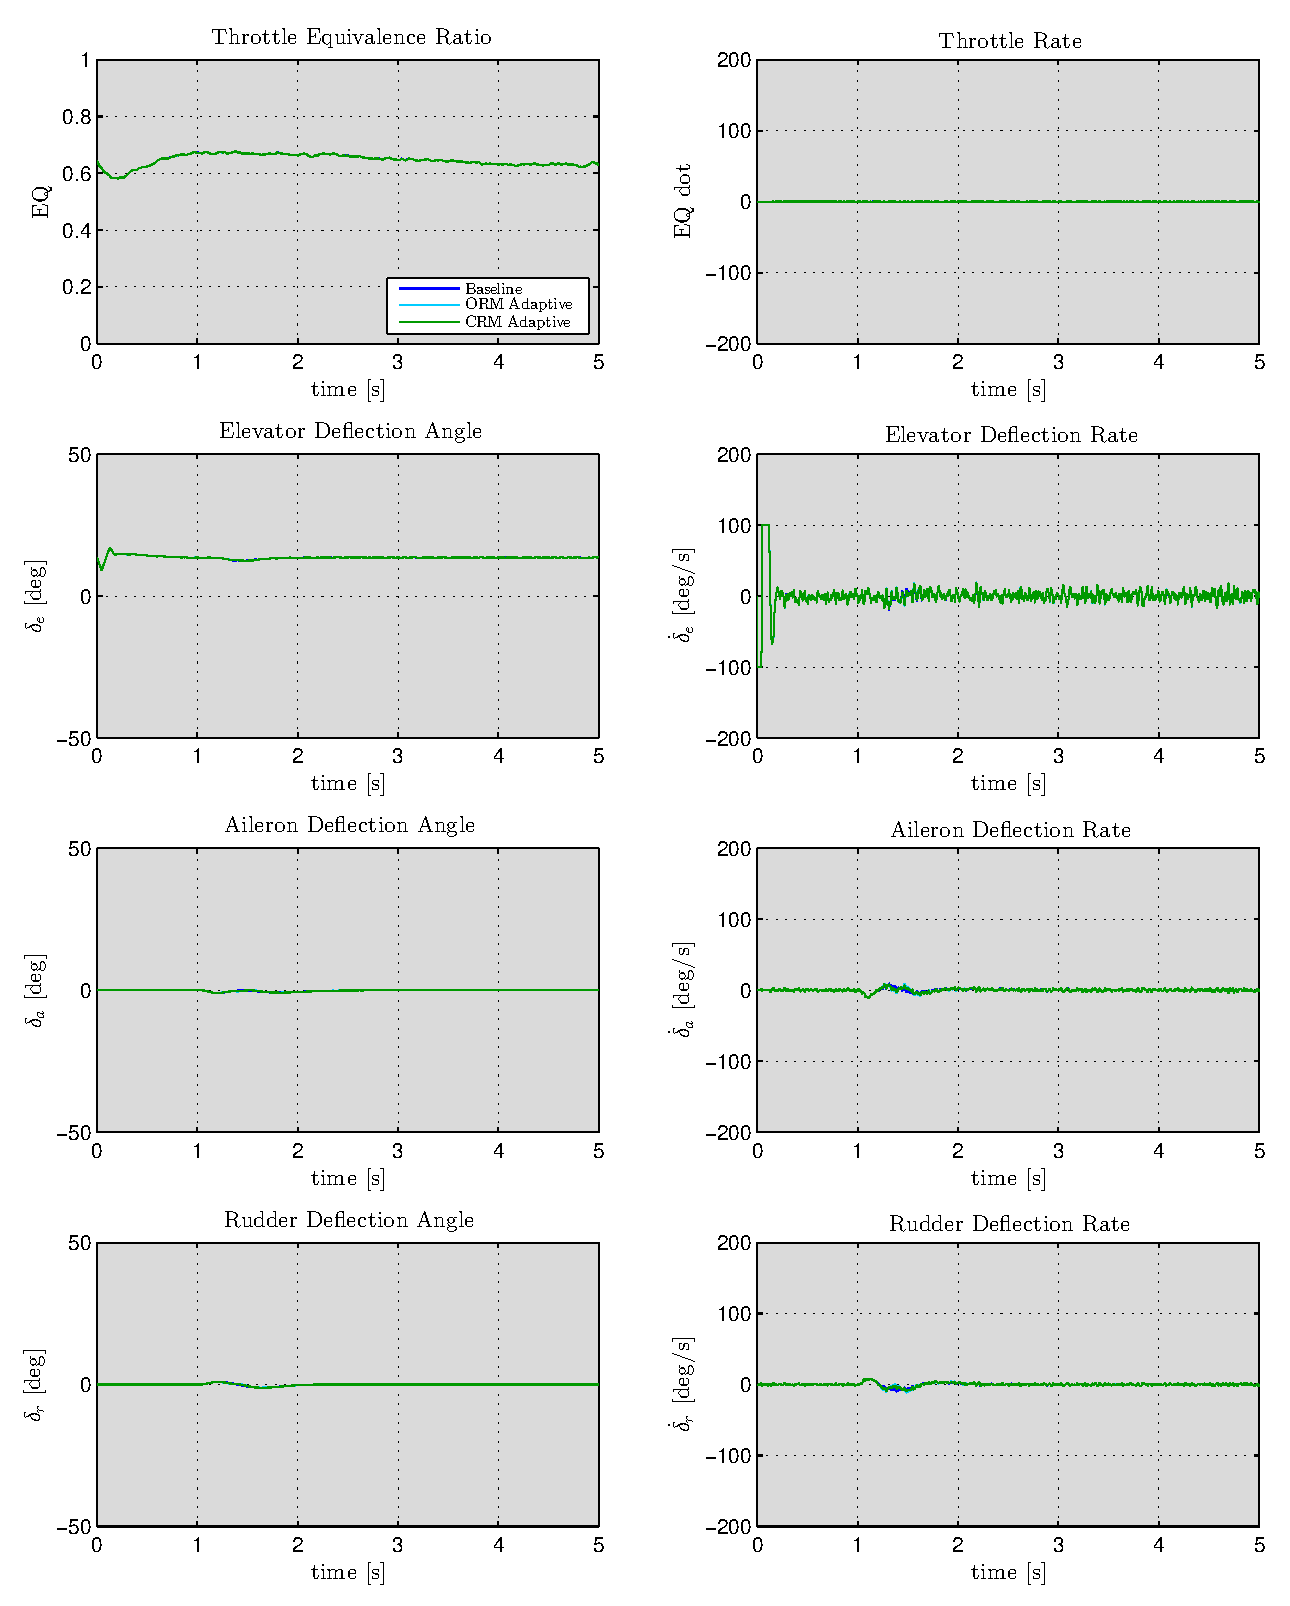
\includegraphics[width=6.5in]{\figurepath/input_latrres_cma400b.eps}
    \caption{2C:\ Input response for pitching moment coefficient scaled $4\times$}
  \end{center}
\end{figure}

\begin{figure}[H]
  \begin{center}
    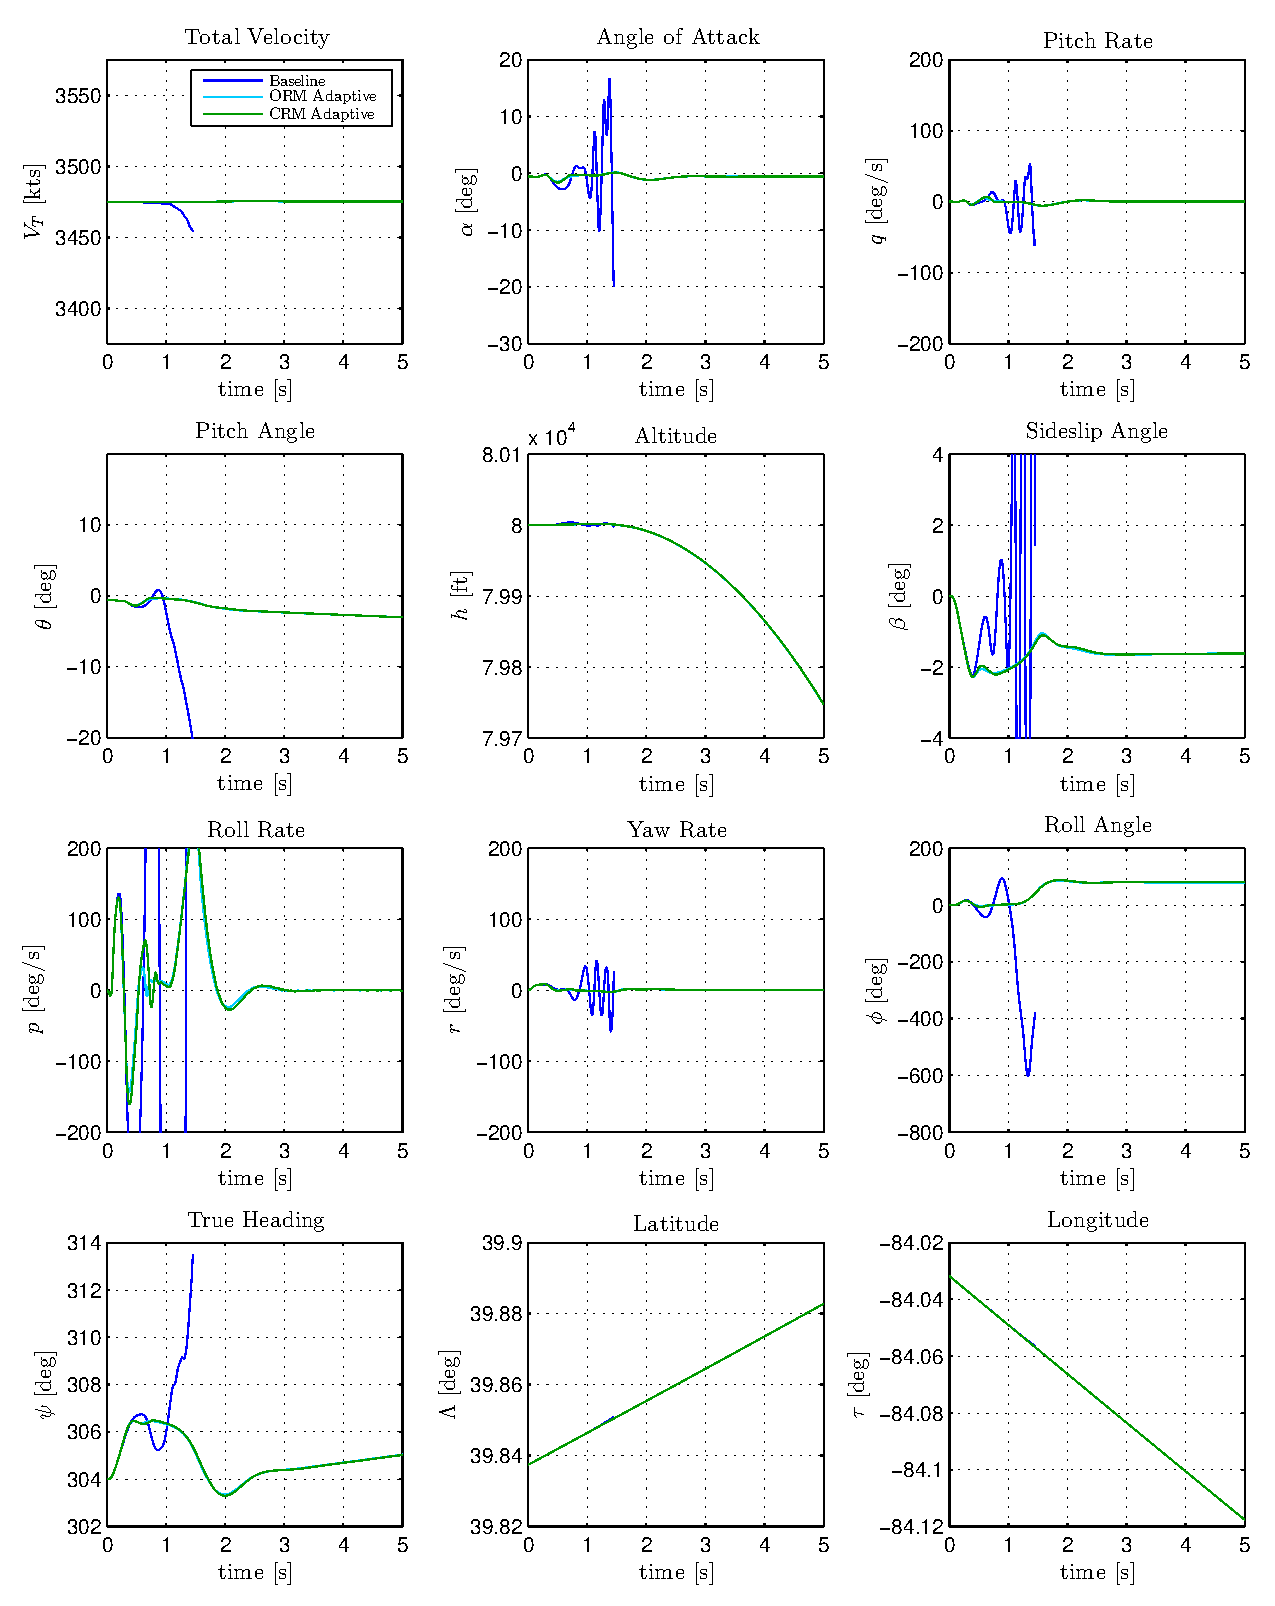
\includegraphics[width=6.5in]{\figurepath/state_latrres_bia016b.eps}
    \caption{2D:\ State response for sensor bias of $+1.6$ degrees on sideslip measurement}
  \end{center}
\end{figure}

\begin{figure}[H]
  \begin{center}
    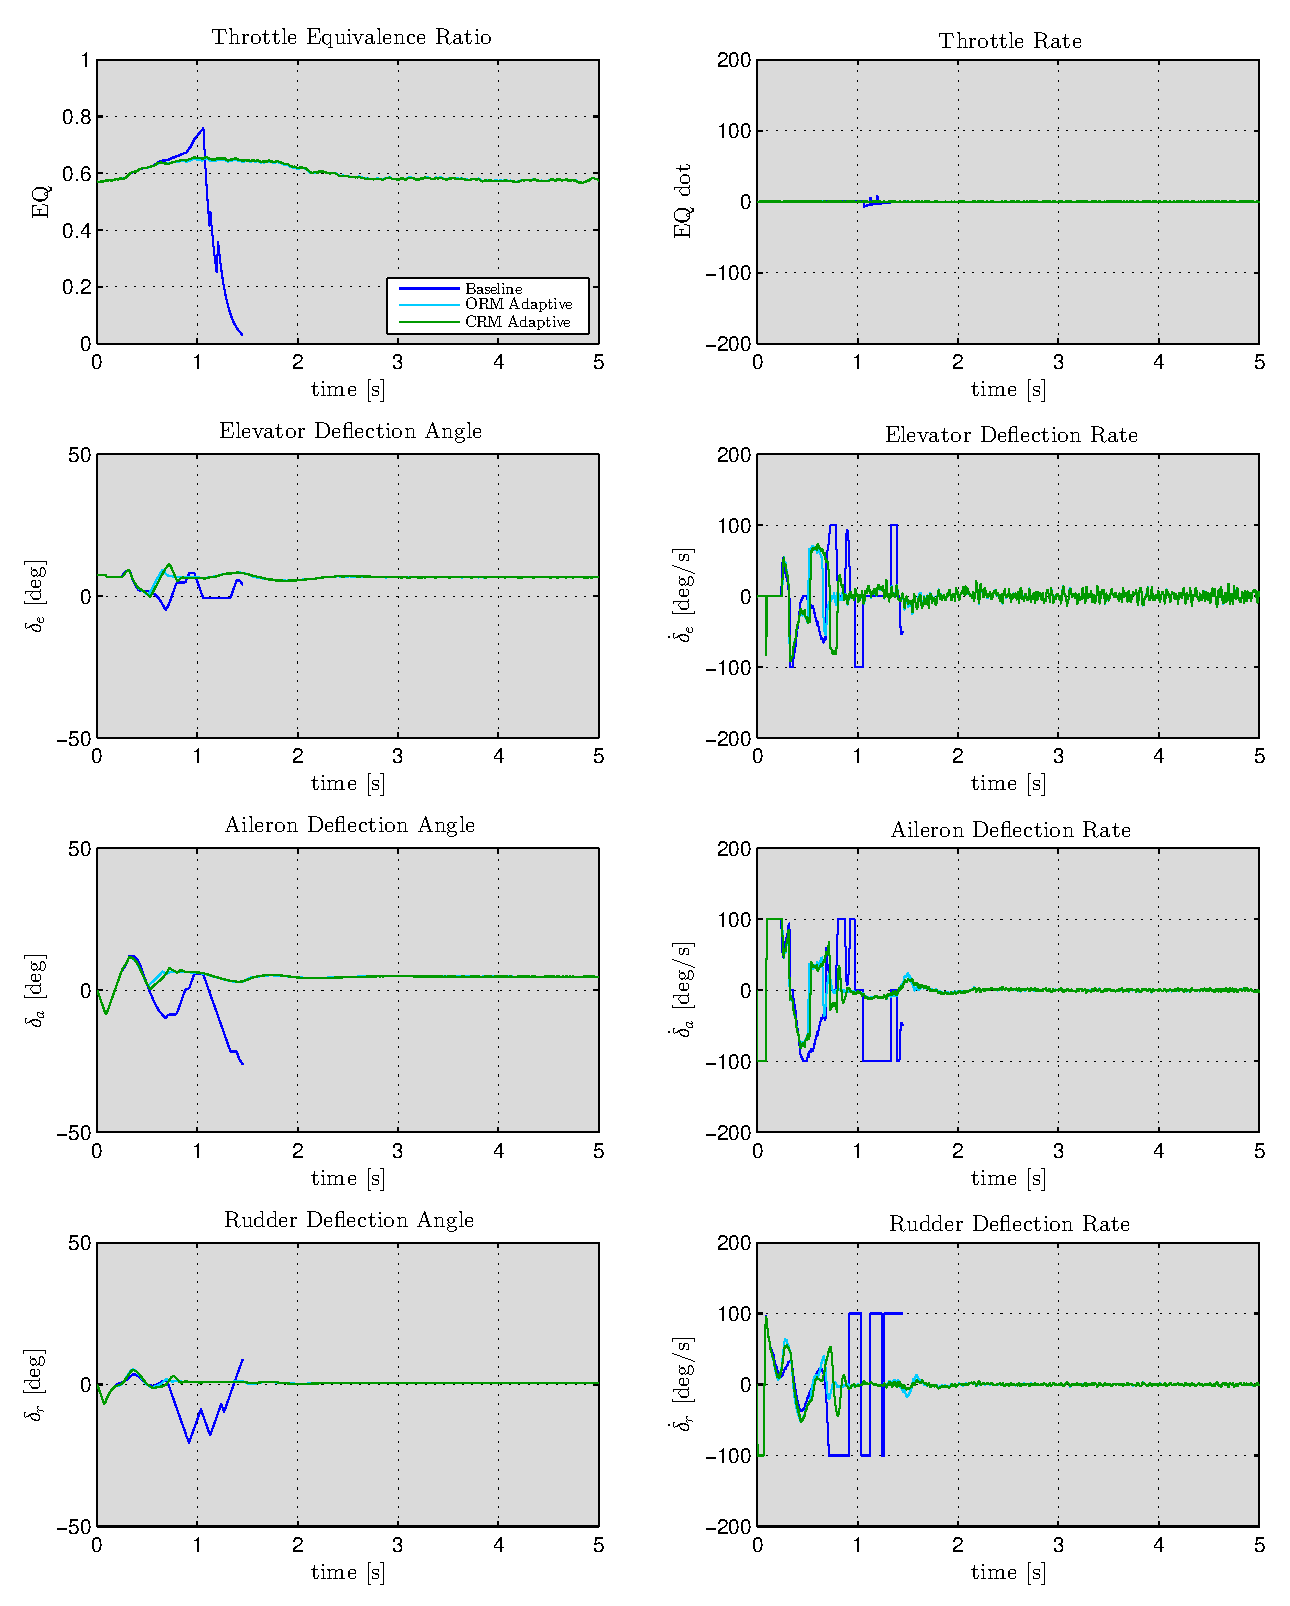
\includegraphics[width=6.5in]{\figurepath/input_latrres_bia016b.eps}
    \caption{2D:\ Input response for sensor bias of $+1.6$ degrees on sideslip measurement}
  \end{center}
\end{figure}
